\documentclass[letterpaper, 12pt]{article}
\usepackage[margin=2cm]{geometry}

\usepackage{amssymb}
\usepackage{graphicx}
\usepackage{subfig}

\setlength{\parindent}{0em}
\setlength{\parskip}{0.5em}

\title{\textbf{18-748 Wireless Sensor Networks Lab 1}}
\author{Emily Ruppel, Iljoo Baek, Mengwen He}

\begin{document}
\maketitle
	
\section{Assignment 2}

\subsection{Data Measurement}

\begin{table}[!h]
	\centering
	\caption{The Measurements of Distance and RSSI}
	\begin{tabular}{|c|c|c|c|c|}
		\hline
		\multicolumn{2}{|c|}{Distance} & \multicolumn{3}{|c|}{RSSI} \\
		\hline
		Yard	&	Meter	&	Min	&	Max	&	Ave.\\
		\hline
		0		&	0		&	39	&	51	&	45	\\
		\hline
		5		&	4.57	&	21	&	25	&	24	\\
		\hline
		10		&	9.14	&	14	&	20	&	18	\\
		\hline
		15		&	13.72	&	7	&	18	&	15	\\
		\hline
		20		&	18.29	&	11	&	14	&	12	\\
		\hline
		25		&	22.86	&	0	&	0	&	0	\\
		\hline
	\end{tabular}
\end{table}

\begin{figure}[!h]
	\centering
	\includegraphics[width=15cm]{./img/data.png}
\end{figure}

\subsection{Compute Path Loss Exponent $n$}

Path loss exponent is given by: $$L=10n\log_{10}d+C$$
\begin{itemize}
	\item $L$: path loss
	\item $n$: path loss exponent
	\item $d$: distance in meters
	\item $C$: system constant
\end{itemize}

From two different data points: $$(L2-L1)=10n\log_{10}(d2/d1) \Rightarrow n=(L2-L1)/(10\log_{10}(d2/d1))$$

As RSSI is linearly related to path loss $$(L2-L1)=(RSSI2-RSSI1)$$

Fix $d1=4.57$, $L1=24$ and get the estimation as Tab.\ref{tab:pathloss}:

\begin{table}[!h]
	\centering
	\caption{The Estimation of Path Loss Exponent}
	\label{tab:pathloss}
	\begin{tabular}{|c|c|c|}
		\hline
		$d2$	&	$L2$	&	$n$	\\
		\hline
		9.14		&	18		&	-1.993	\\
		\hline
		13.72		&	15		&	-1.885	\\
		\hline
		18.29		&	12		&	-1.992	\\
		\hline
		22.86		&	0		&	-3.433 (invalid)	\\
		\hline
	\end{tabular}
\end{table}

Because we cannot get RSSI value when $d2=22.86$, we cannot trust this measurement that just represents the margin of the signal coverage. Therefore, the estimated Path Loss Exponent is:
$$\mathbb{E}[n]=\frac{-1.993-1.885-1.992}{3}=-1.957$$
$$Var[n]=\frac{(1.957-1.993)^2+(1.957-1.885)^2+(1.957-1.992)^2}{3}=0.0039$$
$$\sigma=\sqrt{Var[n]}=0.0621$$

\newpage
\section{Assignment 3}

\subsection{Data Collection}

\begin{figure}[!h]
	\centering
	\subfloat[Case1: Task1 has lower priority.]{\includegraphics[width=3.5cm]{./img/case1_t1.png}\includegraphics[width=3.5cm]{./img/case1_t2.png}}
	~~
	\subfloat[Case2: Task2 has lower priority.]{\includegraphics[width=3.5cm]{./img/case2_t1.png}\includegraphics[width=3.5cm]{./img/case2_t2.png}}
\end{figure}

\subsection{Worst-case Response Time Estimation}

Because the task1 and task2 are released every 1s and 2s, we can directly get their response time from the nanosecond part, and thus easily get the worst-case response time as below:

\begin{itemize}
	\item Case 1:
	\begin{itemize}
		\item Task1: 601562808
		\item Task2: 299804841
	\end{itemize}
	\item Case 2:
	\begin{itemize}
		\item Task1: 298828278
		\item Task2: 601562808
	\end{itemize}
\end{itemize}

\subsection{Explanation of The Differences}

\subsubsection{Response Time}

For case1, because task1 has lower priority, it will be preempted by task2 every 2 seconds; therefore, the response time of task1 is not stable. For case2, because task1 has higher priority, it will not be preempted by task2; therefore, the response time of task1 is stable.

For task2, because its period interval is longer than task1's, and they form a harmonized taskset; therefore, task2's response time is stable for both cases.

\subsubsection{Worst-case Response Time}

Comparing the worst-case response time of task1 and task2 from two cases, we found that the task with higher priority will have smaller worst-case response time.

\subsection{Bonus1: Find a tight CPU reserve budget for each task.}

From the experiment, we know that if task1 with shorter period interval has higher priority, both tasks can have stable response time; therefore, our method is first to use the RMS(Rate-monotonic scheduling) to assign the priority to each task, and then assign each task's reserve budget equals to its worst-case response time.

\newpage
\subsection{Bonus2: Plot graphs for both basks to show their response times.}

\begin{figure}[!h]
	\centering
	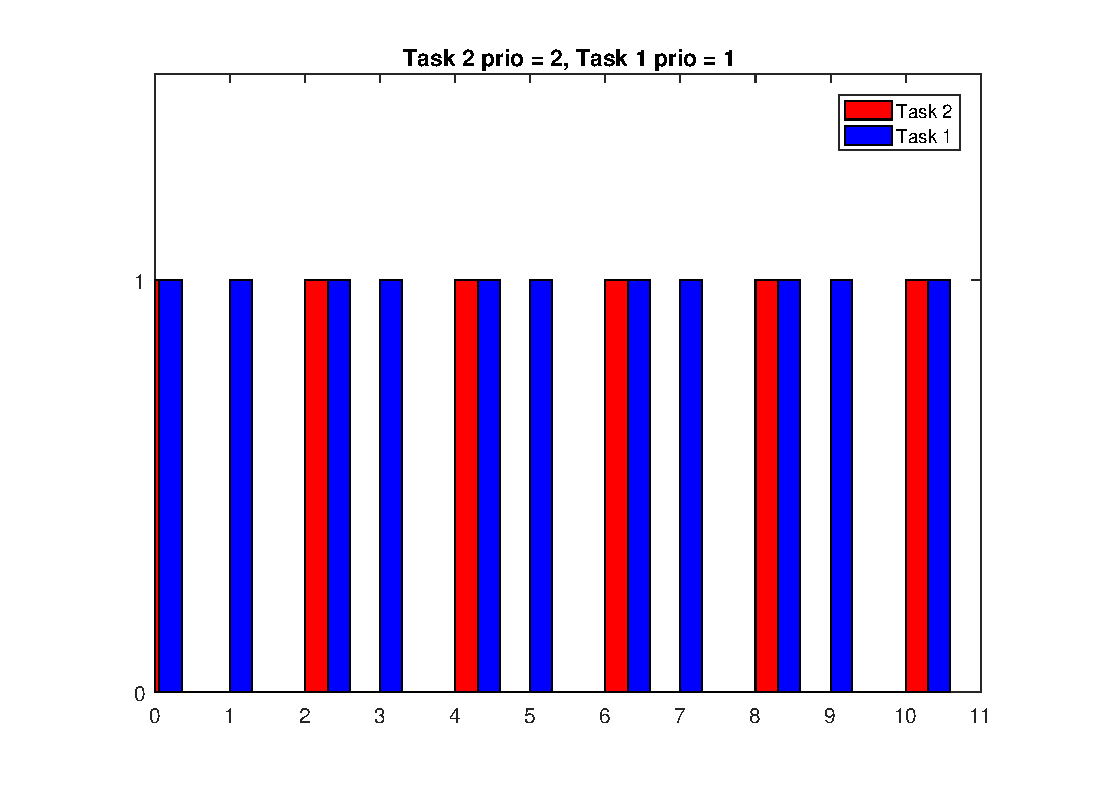
\includegraphics[width=15cm]{./img/Task2_prio2_updated.eps}
	\includegraphics[width=15cm]{./img/Task1_prio2_updated.eps}
\end{figure}


\end{document}\grid
\grid
